%% Untrusted Text, Trusted Tokens: Bounding the Authority of AI Agents in Software Build Pipelines
%% Author: Osita Sean Keluo-Udeke
%% Prepared for: ACM Digital Threats: Research and Practice (DTRAP)
%% Part of the Open Build and Agent Assurance Framework (OBAAF).
%%
%% Build with pdfLaTeX + BibTeX. On Overleaf: New Project > Upload Project > the zip.
%% Requires the acmart class (part of TeX Live; preinstalled on Overleaf).
%%
%% Other venues:
%%   ACM SACMAT 2027 (conference, double-blind): change the class line to
%%     \documentclass[sigconf,review,anonymous]{acmart}
%%   and replace \acmJournal{DTRAP} with
%%     \acmConference[SACMAT '27]{ACM Symposium on Access Control Models and Technologies}{July 19--21, 2027}{Durham, United Kingdom}
%%   The research track allows 10 pages plus 2 pages of references and appendices,
%%   so this full version must be shortened first.
%% For double-anonymous review, add the "anonymous" class option.
\documentclass[acmsmall,screen,review]{acmart}

\acmJournal{DTRAP}
%% Submission copy: no ACM rights block or reference format yet.
\setcopyright{none}
\settopmatter{printacmref=false}
\renewcommand\footnotetextcopyrightpermission[1]{}

\usepackage{tabularx}
\usepackage{xltabular}
\usepackage{pdflscape}
\providecommand{\code}[1]{\texttt{#1}}
%% Large meet operator (n-ary greatest lower bound); defined only if the fonts lack one.
\providecommand{\bigsqcap}{\mathop{\vcenter{\hbox{\Large$\sqcap$}}}}
%% Let TeX stretch spaces a little more before overfilling a line.
\setlength{\emergencystretch}{1.5em}

\begin{document}

\title[Untrusted Text, Trusted Tokens]{Untrusted Text, Trusted Tokens: Bounding the Authority of AI Agents in Software Build Pipelines}

\author{Osita Sean Keluo-Udeke}
\affiliation{%
  \institution{Affiliation to be confirmed}
  \city{Austin}
  \state{Texas}
  \country{USA}}
\email{seankudeke@gmail.com}

\renewcommand{\shortauthors}{Keluo-Udeke}

\begin{abstract}
Large language model (LLM) agents now run inside CI/CD pipelines, where they triage issues, review pull requests, repair builds, and commit code. They read text that anyone can write while holding credentials that can change source code and releases. This breaks a separation that build security has long relied on: untrusted input is data, never instructions.

This paper develops the agent-assurance component of the Open Build and Agent Assurance Framework (OBAAF), an open framework for securing build pipelines and the AI agents that operate in them. Ten documented incidents and disclosures from 2025–2026 show three recurring root causes: untrusted text reaching a privileged agent, credentials broader or longer-lived than the task needed, and no binding between what an agent read, what it could do, and what it changed. We propose \emph{taint-bounded authority}, adapted from Biba's low-water-mark policy: an agent invocation's authority must never exceed the trust level of the least-trusted principal able to influence its context. From it we derive eight control requirements and a three-lane reference architecture built from existing CI primitives, including a signed attestation of each agent run.

Under stated assumptions, an adversary who can only write public text gains no authority through the agent. Analytically, the requirements would have prevented the harmful outcome in eight of the ten cases and at least contained it in the other two. We trace them to NIST's SSDF, NIST SP 800-204D, SLSA, and NIST's 2026 questions on agent identity and authorization, assess deployability on GitHub Actions, and give a protocol for empirical validation.
\end{abstract}

%% CCS concepts: confirm or regenerate at https://dl.acm.org/ccs before submission.
\ccsdesc[500]{Security and privacy~Software security engineering}
\ccsdesc[300]{Security and privacy~Access control}
\ccsdesc[300]{Security and privacy~Information flow control}
\ccsdesc[100]{Computing methodologies~Intelligent agents}

\keywords{software supply chain security, CI/CD, LLM agents, prompt injection, integrity models, provenance}

\maketitle

\section{Introduction}\label{sec:1}

Software teams have begun to place LLM agents inside the automation that builds and ships their code. GitHub's Copilot cloud agent takes assigned tasks and opens pull requests from a branch of its own~\cite{githubndrisks}. Anthropic's Claude Code action, Google's Gemini CLI, and OpenAI's Codex are invoked from workflow files in response to issues, comments, and pull requests~\cite{anthropicndsecurity,daelman2025prompt}. A May 2026 measurement found 13,392 workflows that invoke agents across 10,792 repositories, and 1,033 AI-assisted actions in the GitHub Marketplace~\cite{wang2026demystifying}.

The risks are no longer hypothetical. In December 2025, researchers showed on a private test fork that text in issues and pull requests could direct agents running in GitHub Actions to expose the tokens and credentials their workflows hold, and reported vulnerable workflows at five or more Fortune 500 companies~\cite{daelman2025prompt}. The May 2026 measurement confirmed 496 exploitable agentic workflow injection flaws, and found that only 21 of the 1,033 AI-assisted actions provided explicit caller-identity access control~\cite{wang2026demystifying}. Even that control is not enough. A disclosed flaw in one widely used action let an outside contributor rewrite a pull-request title after a maintainer had invoked the agent but before the agent read it~\cite{stawinski2026trusting}. In February 2026 an attacker went further: an issue title steered an AI triage workflow into running code, which poisoned a build cache shared with release jobs and ended in an unauthorized package release (\S\ref{sec:4}).

Agents differ from earlier pipeline automation in one decisive way. A conventional workflow parses an issue title as data. When it fails to, for instance by interpolating the title into a shell command, the result is a well-understood injection flaw that analysis tools can find and engineers can fix~\cite{lobavcevski2021keeping,koishybayev2022characterizing,muralee2023argus}. An agent, by contrast, is built to treat text as instructions. Any text that reaches its context can steer what it does next, and the research literature offers no reliable way to prevent this at the model. Indirect prompt injection was demonstrated against deployed applications in 2023~\cite{greshake2023not}, and in 2025 adaptive attacks bypassed twelve published defenses, most with success rates above 90\%~\cite{nasr2025attacker}. Once untrusted text and privileged credentials share an agent's context, the credentials are, in effect, available to whoever wrote the text~\cite{willison2025lethal}.

Public guidance is only beginning to respond. NIST's National Cybersecurity Center of Excellence (NCCoE) opened a project on agent identity and authorization in February 2026, asking how agents should be identified, authorized, audited, and protected from prompt injection~\cite{booth2026accelerating}, as part of a broader NIST initiative on agent standards~\cite{national2026announcing}.

We take a systems view. Rather than ask the model to resist injection, we ask what authority an agent invocation may safely hold, given who could have written its inputs. The answer comes from integrity models that predate LLMs by decades. Biba's low-water-mark policy lowers a subject's integrity to that of the least trustworthy data it reads~\cite{biba1977integrity}. Clark and Wilson's model lets untrusted data become trusted only through a certified procedure with separation of duty~\cite{clark1987comparison}. Applied to CI, these models yield a simple rule and an architecture that can be built today. Our requirements complement NIST's Secure Software Development Framework (SSDF)~\cite{souppaya2022secure,booth2025secure}, NIST's guidance on securing CI/CD pipelines in SP 800-204D~\cite{chandramouli2024strategies}, and the SLSA framework~\cite{openndslsa}. Those frameworks protect source, builds, and provenance, but they predate agents in build systems and do not address what an automated actor may do after reading untrusted text.

This paper develops the agent-assurance component of the Open Build and Agent Assurance Framework (OBAAF) and makes five contributions:

\begin{enumerate}
\item A system and threat model for agentic build pipelines (\S\ref{sec:3}). It treats the model as fully controllable by any text in its context, and identifies the input channels, credentials, and effects that matter.
\item An analysis of ten documented incidents and disclosures from 2025–2026 (\S\ref{sec:4}), which identifies three recurring root causes.
\item \emph{Taint-bounded authority} (\S\ref{sec:5}), a principle that bounds an agent invocation's authority by the trust level of the least-trusted principal able to influence its context. A short argument shows that, under stated assumptions, an adversary gains no authority through the agent.
\item Eight control requirements (\S\ref{sec:6}) and a reference architecture that realizes them with existing CI primitives (\S\ref{sec:7}).
\item An analytical evaluation (\S\ref{sec:8}), covering incident coverage, traceability to the SSDF, SLSA, and the NCCoE questions, and deployability on GitHub Actions, plus a protocol for empirical validation (\S\ref{sec:9}).
\end{enumerate}

\emph{Scope.} We address agents that run inside build pipelines or act on repositories through pipeline credentials. The incident analysis also includes developer-side assistants, because they share the same failure pattern. Endpoint security, model training, and compromise of model providers are out of scope. A companion paper~\cite{keluoudeke2026securing} develops OBAAF's build-assurance component for video game studios: a sector profile of the SSDF and SLSA that incorporates these requirements, and a self-assessment for small studios.


\section{Background}\label{sec:2}


\subsection{Build pipelines as planes of authority}\label{sec:2.1}

A modern CI/CD pipeline can be described as five planes, each with its own principals and protections. The \emph{source plane} holds repositories and their protected branches. The \emph{trigger plane} turns events (pushes, pull requests, issues, comments, schedules) into workflow runs. The \emph{execution plane} runs jobs on runners, which may be ephemeral virtual machines or persistent hosts. The \emph{credential plane} supplies the identities those jobs use: a job token issued by the platform, short-lived cloud credentials, registry tokens, and signing keys. The \emph{release plane} signs and publishes artifacts and records how they were built.

Supply chain integrity frameworks protect these planes. in-toto binds each step of a pipeline to signed metadata about its inputs and outputs, so that a verifier can check that an artifact passed through the intended steps~\cite{torresarias2019toto}. Sigstore removed most of the key-management burden from signing by issuing short-lived certificates bound to workload identities~\cite{newman2022sigstore}. SLSA defines levels of build integrity. At Build Level 3 it requires a fresh, isolated build environment for every build, and provenance that user-defined build steps cannot forge, because signing material must not be accessible to them~\cite{openndslsa}. Platforms have adopted these ideas. GitHub issues each job an OpenID Connect (OIDC) token whose claims name the repository, ref, environment, and workflow, which cloud providers exchange for credentials that expire with the job~\cite{githubndopenid}. It made the default job token read-only for new repositories in February 2023~\cite{github2023github}, releases environment secrets only after required reviewers approve~\cite{githubnddeployments}, and generates signed in-toto attestations, including attestations with custom predicate types~\cite{githubndactions}.


\subsection{How pipelines are attacked}\label{sec:2.2}

Taxonomies of supply chain attacks catalog 107 attack vectors across contribution, build, and distribution~\cite{ladisa2023sok}, and frame defenses around transparency, validity, and separation~\cite{okafor2022sok}. CI services in particular expose risk through over-privileged tokens, execution of untrusted code, and third-party plugins: a 2022 study of 447,238 GitHub workflows found 99.8\% held read-write repository access~\cite{koishybayev2022characterizing}, and a 2023 study characterized similar weaknesses across CI services~\cite{gu2023continuous}.

Two failure patterns recur. The first is untrusted input flowing into a privileged context. GitHub's \code{pull\_\allowbreak{}request\_\allowbreak{}target} trigger runs with the base repository's write token and secrets, so checking out and executing a pull request's code under it can compromise the repository~\cite{lobavcevski2021keeping}. Static analysis has found code injection flaws of this kind in 4,307 workflows~\cite{muralee2023argus}. The second is compromise of components the pipeline trusts. In March 2025, the tj-actions/changed-files action, used by more than 23,000 repositories, was altered to dump runner secrets into build logs~\cite{stepsecurity2025harden}. The August 2025 attack on the Nx build system combined both patterns. An injection in a workflow that checked pull-request titles yielded a write-capable token, which the attacker used to trigger the project's publishing workflow and steal its registry token~\cite{nx2025s1ngularity}.


\subsection{Agents in CI and prompt injection}\label{sec:2.3}

An agent couples a model with a harness that assembles context and executes tool calls: shell commands, repository API calls, and, increasingly, calls to Model Context Protocol (MCP) servers~\cite{model2025security}. In CI, the context is assembled from the triggering event, repository files, tool outputs, and fetched content. The Open Worldwide Application Security Project (OWASP) lists prompt injection and excessive agency among the top risks for LLM applications~\cite{owaspndowasp}.

Indirect prompt injection, in which instructions are placed in data a model later reads, was demonstrated against deployed systems in 2023~\cite{greshake2023not}. Benchmarks such as AgentDojo now measure agent robustness across 97 tasks and 629 security test cases~\cite{debenedetti2024agentdojo}. Model-level defenses mark untrusted input so that the model can recognize it~\cite{hines2024defending}, or train models to prioritize privileged instructions~\cite{wallace2024instruction}. Adaptive attacks, however, have defeated most published defenses~\cite{nasr2025attacker}. We therefore treat model-level defenses as useful but insufficient, and look to system design.


\subsection{Integrity and authority}\label{sec:2.4}

Three classical ideas underpin our design. Saltzer and Schroeder's principles of least privilege, separation of privilege, and complete mediation describe how authority should be granted and checked~\cite{saltzer1975protection}. Hardy's \emph{confused deputy}, a program that misuses authority it holds for one party at the request of another~\cite{hardy1988confused}, is the exact shape of an injected agent. Integrity models make trust flow explicit. Denning's lattice model formalizes information flow among security classes~\cite{denning1976lattice}. Biba's integrity model forbids a high-integrity subject from reading low-integrity data; its low-water-mark variant instead lowers the subject's integrity to the lowest level it has read~\cite{biba1977integrity}. Clark and Wilson's model requires that unconstrained data become trusted only through certified transformation procedures, with separation of duty~\cite{clark1987comparison}. Section~\ref{sec:5} applies these models to agent invocations.


\section{System and threat model}\label{sec:3}


\subsection{System model}\label{sec:3.1}

We model an agentic build pipeline in terms of principals, content, agent invocations, and capabilities. Figure~\ref{fig:1} shows how they relate.

\begin{itemize}
\item \emph{Principals} are the parties whose actions or words can enter the pipeline: the public (anyone who can open an issue or a pull request from a fork), contributors with limited rights, maintainers who can merge to protected branches, release authorities who can approve publication, and the suppliers of tools, actions, containers, and models.
\item \emph{Content} is anything an agent can read: event payloads (issue bodies, pull-request titles and descriptions, comments, branch names, commit messages), repository files, build and test output, fetched web pages, and the outputs of tools and MCP servers.
\item An \emph{agent invocation} is one run of an agent inside a CI job. It has a \emph{context}, the content it reads during the run, and an \emph{authority}, the set of capabilities reachable from its environment.
\item A \emph{capability} is an effect the invocation can cause: reading private source or a secret, writing to a branch, editing workflow or instruction files, calling an API with a credential, publishing an artifact, or sending data over the network.
\end{itemize}

Authority includes \emph{ambient authority}: capabilities present in the environment that the task did not ask for. Runners differ in how much they carry over. Each GitHub-hosted runner, except single-CPU runners, is a new virtual machine~\cite{githubndgithub}, whereas a self-hosted runner retains state between jobs unless it is configured to be ephemeral. Within a job, ambient authority includes secrets exported as environment variables, a repository token persisted in the workspace's git configuration (the default behavior of GitHub's checkout action~\cite{githubndactionsa}), cloud metadata endpoints, caches that release jobs later read, and unrestricted network egress.

\begin{figure}[htbp]
\centering
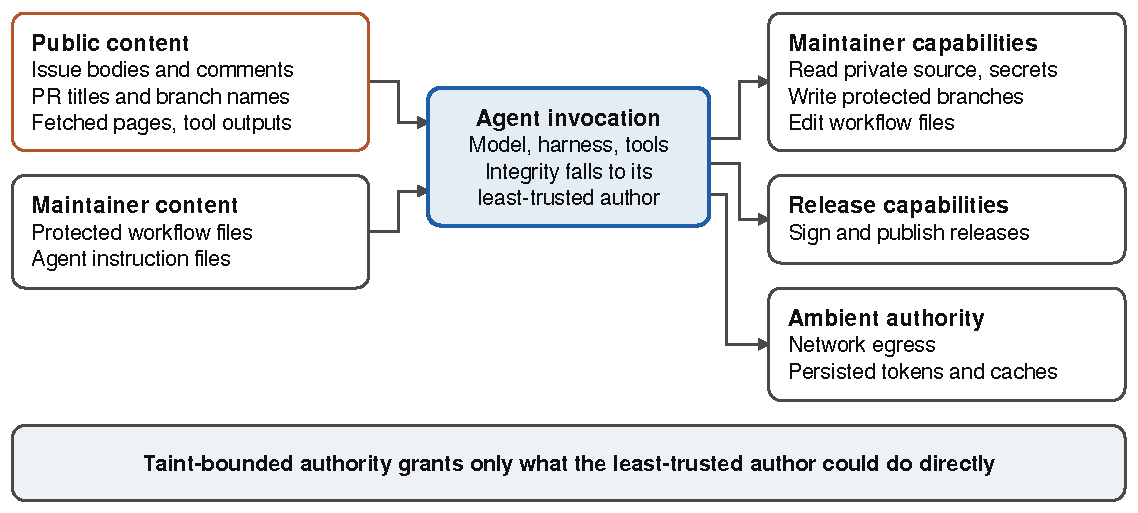
\includegraphics[width=\linewidth]{figures/fig1-authority.pdf}
\caption{Content an agent reads, grouped by who can write it (left), and the authority present in its environment (right). Without a bound, text from the least-trusted author can direct every capability on the right.}
\Description{A diagram with three columns. Left: public content (issue bodies, pull-request titles, fetched pages) and maintainer content (protected workflow and agent instruction files) both flow into an agent invocation in the middle. Right: the agent can exercise maintainer capabilities, release capabilities, and ambient authority such as network egress and persisted tokens. A banner states that taint-bounded authority grants only what the least-trusted author could do directly.}
\label{fig:1}
\end{figure}


\subsection{Trust levels}\label{sec:3.2}

We order principals by the trust a project places in them, forming a chain \emph{Public} $\sqsubseteq$ \emph{Contributor} $\sqsubseteq$ \emph{Maintainer} $\sqsubseteq$ \emph{Release}. Each principal \emph{p} has a level $\ell$(\emph{p}). Each capability \emph{c} has a \emph{required level} req(\emph{c}): the lowest level whose holders may cause \emph{c} directly under the project's own rules.

\begin{center}
\small
\begin{tabularx}{\linewidth}{@{}>{\hsize=1.665\hsize\raggedright\arraybackslash}X>{\hsize=0.335\hsize\raggedright\arraybackslash}X@{}}
\toprule
\textbf{Capability} & \textbf{Typical required level} \\
\midrule
Comment on a public issue; open a pull request from a fork & Public \\
Push to a non-protected branch; apply labels & Contributor \\
Merge to a protected branch; edit workflow or agent-instruction files; read repository secrets & Maintainer \\
Approve or publish a release; use a signing key & Release \\
\bottomrule
\end{tabularx}
\end{center}

Reading private source has the level of the principals entitled to read it. Suppliers are placed by policy. A first-party action pinned by digest and verified against its provenance may be trusted at Maintainer level, whereas the tool descriptions and outputs of an arbitrary MCP server are Public content.


\subsection{Adversaries and goals}\label{sec:3.3}

We consider three adversaries.

\begin{itemize}
\item \emph{A1, outside author.} Can create or edit text in any channel open to the public: issues, comments, pull requests and their titles and branch names, and commits in forks. Cannot push to the base repository. This adversary drove most of the incidents in \S\ref{sec:4}.
\item \emph{A2, upstream supplier.} Controls content an agent ingests indirectly: a dependency's README or source comments, a web page the agent fetches, an MCP server's tool descriptions and outputs, or an action or container the pipeline runs.
\item \emph{A3, low-privilege insider.} Holds Contributor rights, for example the ability to push non-protected branches or label issues, and seeks effects that require Maintainer or Release level.
\end{itemize}

The adversary's goals are (G1) disclosure of secrets or private source; (G2) tampering with protected branches or released artifacts; (G3) persistence, such as editing workflow or agent-instruction files, or poisoning caches that later runs consume; (G4) repudiation, that is, causing effects that cannot be attributed to their true origin; and (G5) resource abuse.

\emph{Trust assumptions.} We trust the CI platform's isolation between jobs, its enforcement of token scopes and environment protection rules, and the cryptographic primitives behind signing and OIDC. We do not trust the model. We adopt a \emph{worst-case model assumption}: once content written by a principal is in an invocation's context, that principal may be able to direct every subsequent action of the invocation. The assumption is pessimistic, but it is the only one current evidence supports~\cite{nasr2025attacker}. It matches the position of recent work on agent design patterns, which holds that an agent that has ingested untrusted input must be constrained so that the input cannot trigger consequential actions~\cite{beurerkellner2025design}. Compromise of the CI platform itself, of model providers, and of developer endpoints is out of scope.


\section{Analysis of documented incidents}\label{sec:4}


\subsection{Method}\label{sec:4.1}

We collected publicly documented incidents and vulnerability disclosures from January 2025 through May 2026 that met either of two conditions. In the first, an AI agent or assistant operating on a software repository or in a build pipeline was induced to act against its operator. In the second, a build pipeline delivered attacker-controlled agent instructions or was used to abuse agent tooling. Sources were vendor advisories, researcher write-ups, and project postmortems, and we read each primary source. We included a case if its source described the entry channel, the authority abused, and the outcome. Ten cases met these criteria (Table~\ref{tab:1}).

For each case we coded the setting, entry channel, authority abused, outcome, and whether the attack was exploited in the wild or demonstrated by researchers. We then coded root causes using three categories that emerged from the cases:

\begin{itemize}
\item \emph{RC1, input–authority mismatch.} Text from a principal less trusted than the authority it could direct reached the agent's context.
\item \emph{RC2, excess standing authority.} Credentials, tools, or network access were broader or longer-lived than the task needed.
\item \emph{RC3, unbound effects.} Nothing bound the agent's inputs, granted authority, and resulting changes into a record that could be verified later.
\end{itemize}

\begin{landscape}
\begingroup
\scriptsize
\begin{xltabular}{\linewidth}{@{}>{\hsize=0.905\hsize\raggedright\arraybackslash}X>{\hsize=0.724\hsize\raggedright\arraybackslash}X>{\hsize=1.214\hsize\raggedright\arraybackslash}X>{\hsize=1.419\hsize\raggedright\arraybackslash}X>{\hsize=1.419\hsize\raggedright\arraybackslash}X>{\hsize=0.838\hsize\raggedright\arraybackslash}X>{\hsize=0.482\hsize\raggedright\arraybackslash}X@{}}
\caption{Documented incidents and disclosures, in order of disclosure.}\label{tab:1}\\
\toprule
\textbf{Case (disclosed)} & \textbf{Setting} & \textbf{Entry channel} & \textbf{Authority abused} & \textbf{Outcome} & \textbf{Status} & \textbf{Root causes} \\
\midrule
\endfirsthead
\multicolumn{7}{@{}l}{\emph{Table~\ref{tab:1}, continued}}\\
\toprule
\textbf{Case (disclosed)} & \textbf{Setting} & \textbf{Entry channel} & \textbf{Authority abused} & \textbf{Outcome} & \textbf{Status} & \textbf{Root causes} \\
\midrule
\endhead
\bottomrule
\endlastfoot
Rules File Backdoor \cite{pillar2025new} (Mar 2025) & Coding assistants in IDEs & Hidden Unicode instructions in shared rules files & The assistant's ability to write code into the developer's project & Attacker-chosen code suggested, with instructions to hide the change from the chat log & Demonstrated & RC1, RC3 \\
GitHub MCP \cite{invariant2025github} (May 2025) & Developer agent using a GitHub MCP server & Malicious issue in a public repository & Token with read access to the user's private repositories; pull-request creation & Private repository data published in a public pull request & Demonstrated & RC1, RC2 \\
GitLab Duo \cite{mayraz2025remote} (May 2025) & Assistant built into a DevOps platform & Hidden prompts in merge requests, comments, commit messages, issues, and source files & The viewing user's access to private projects; HTML in streamed responses & Private source code sent out through image requests & Demonstrated & RC1, RC2 \\
Gemini CLI \cite{cox2025code} (Jul 2025) & Command-line coding agent & Instructions in README.md and GEMINI.md of an untrusted codebase & Shell commands approved by matching an allow-listed prefix & Chained commands ran silently; environment variables exfiltrated & Demonstrated & RC1, RC2 \\
Amazon Q extension \cite{amazon2025security} (Jul 2025) & Release pipeline of an agent product & Code committed with an over-scoped token from the build configuration & Write access to the source repository; automatic inclusion in a release & Malicious code shipped in version 1.84.0, though a syntax error stopped it from running & Exploited & RC2, RC3 \\
Nx ``s1ngularity'' \cite{nx2025s1ngularity} (Aug 2025) & CI workflow; malware that invoked local AI tools & Unsanitized pull-request title in a \code{pull\_\allowbreak{}request\_\allowbreak{}target} workflow & Read-write job token; publishing workflow holding a registry token & Malicious packages live for about four hours; the payload used local AI tools to search for secrets & Exploited & RC1, RC2, RC3 \\
CamoLeak \cite{mayraz2025camoleak} (Oct 2025) & Chat assistant on a code-hosting platform & Hidden comments in pull-request descriptions & The viewing user's access to private repositories; image rendering through the platform's own proxy & Secrets and private code exfiltrated through pre-signed proxy URLs & Demonstrated & RC1, RC2 \\
PromptPwnd \cite{daelman2025prompt} (Dec 2025) & Agent actions in GitHub Actions & Issue and pull-request text inserted into prompts & Write-capable job token; cloud and model API keys; shell and issue-editing tools & Credentials written into an issue body on a test fork; vulnerable workflows reported at five or more Fortune 500 companies & Demonstrated & RC1, RC2 \\
Claude Code action \cite{stawinski2026trusting} (Feb 2026) & Agent action in GitHub Actions & Pull-request title changed after a maintainer invoked the agent & Job token, secrets, OIDC roles, and the runner & Code execution in the workflow, exposing secrets and push access & Demonstrated & RC1, RC2 \\
Clinejection \cite{khan2026clinejection} (Feb 2026) & AI issue-triage workflow in GitHub Actions & Instructions in an issue title; any GitHub user could trigger the workflow & Shell and file tools; a build cache shared with release workflows & Cache poisoned and publishing tokens stolen; an unauthorized package version was live for about eight hours & Exploited & RC1, RC2, RC3 \\
\end{xltabular}
\endgroup
\end{landscape}


\subsection{Findings}\label{sec:4.2}

\emph{Input–authority mismatch is structural.} RC1 appears in nine of the ten cases. In each, the principal who controlled the text was less trusted than the authority the text could direct. The pattern holds across IDE assistants, chat assistants, command-line agents, and CI actions, which suggests it is a property of the architecture rather than a defect of particular products. Two of the disclosures say as much: one calls the problem an architectural issue at the level of the agent system~\cite{invariant2025github}, and another concludes that any system letting an LLM ingest user-controlled content must treat that content as untrusted~\cite{mayraz2025remote}.

\emph{Invoker checks do not establish context trust.} The Claude Code action verified that the person who invoked it had write access, but the text the model read was written, and later modified, by an outside contributor~\cite{stawinski2026trusting}. Copilot's cloud agent takes a stronger position: comments from users without write access are never presented to the agent~\cite{githubndrisks}. Across the ecosystem, explicit caller-identity checks appeared in only 21 of 1,033 AI-assisted actions~\cite{wang2026demystifying}. The Cline workflow removed the check altogether, letting any GitHub user trigger an agent that held shell access~\cite{khan2026clinejection}. What matters is not who invoked the agent but who wrote what it reads.

\emph{Once private data is in reach, exfiltration channels are everywhere.} Data left through a public pull request~\cite{invariant2025github}, rendered images~\cite{mayraz2025remote}, the platform's own image proxy~\cite{mayraz2025camoleak}, and an edit to an issue~\cite{daelman2025prompt}. Allow-listing destinations would not have helped where the destination was the hosting platform itself. Such channels cannot be closed one at a time. The reliable control is to keep private data out of reach of any invocation that untrusted text can steer, which, as \S\ref{sec:5} shows, is the confidentiality side of the same principle.

\emph{Automated paths reached releases.} In three cases, Amazon Q, Nx, and Cline, attacker-controlled code reached a published release through an automated path. Each project's remediation moved toward the controls we propose: revoking and replacing credentials and withdrawing the affected version~\cite{amazon2025security}; publishing through OIDC-based trusted publishing, with manual approval of releases and added provenance checks~\cite{nx2025s1ngularity}; and removing the agent workflow, keeping caches out of workflows that handle credentials, and moving to OIDC-based publishing~\cite{cline2026post}.


\section{Taint-bounded authority}\label{sec:5}


\subsection{Definitions}\label{sec:5.1}

Let \emph{L} be the trust levels of \S\ref{sec:3.2}, ordered by $\sqsubseteq$, with meet $\sqcap$ (the lower of two levels). For an agent invocation $\alpha$:

\begin{itemize}
\item \emph{Inf}($\alpha$) is the set of principals able to influence any content in $\alpha$'s context before $\alpha$ reads it. A principal influences content if it wrote any part of it, could have modified it between the moment authority was decided and the moment the content was read, or controls the source from which it was fetched.
\item \emph{I}($\alpha$), the \emph{integrity level} of $\alpha$, is the level of its least-trusted influencer: the meet of $\ell$(\emph{p}) over all \emph{p} in \emph{Inf}($\alpha$).
\item \emph{A}($\alpha$), the \emph{authority} of $\alpha$, is every capability reachable from its environment, including ambient authority.
\end{itemize}


\subsection{The principle}\label{sec:5.2}

\emph{Taint-bounded authority} requires that every capability an invocation can exercise be one its least-trusted influencer could exercise directly:

\begin{equation}\label{eq:tba}
\forall c \in A(\alpha):\quad \mathrm{req}(c) \sqsubseteq I(\alpha) = \bigsqcap_{p \in \mathit{Inf}(\alpha)} \ell(p)
\end{equation}

Put differently, adding text to an agent's context must never add authority. This is Biba's low-water-mark policy for subjects~\cite{biba1977integrity}, with ``write'' generalized to any effect. The generalization includes reads of secrets and private source, because in an agentic setting reading data is the precondition for leaking it through whatever output channel the agent has. The principle states formally what practitioners have begun to say informally: an LLM should have no more agency than anyone or anything that can invoke it~\cite{stawinski2026trusting}. We strengthen \emph{invoke} to \emph{influence}, because the cases in \S\ref{sec:4} show that the invoker is often not the author of what the model reads.


\subsection{What it guarantees}\label{sec:5.3}

\emph{Proposition.} Assume (i) \emph{complete mediation}: every effect of $\alpha$ requires a capability in \emph{A}($\alpha$), with no ambient authority outside it; and (ii) \emph{sound labeling}: \emph{Inf}($\alpha$) includes every principal able to influence $\alpha$'s context. If $\alpha$ satisfies taint-bounded authority and an adversary at level \emph{a} influences $\alpha$, then every effect $\alpha$ can cause is one the adversary could cause directly.

\emph{Argument.} The adversary is in \emph{Inf}($\alpha$), so \emph{I}($\alpha$) $\sqsubseteq$ \emph{a}. Taint-bounded authority gives req(\emph{c}) $\sqsubseteq$ \emph{I}($\alpha$) for every \emph{c} in \emph{A}($\alpha$), and hence req(\emph{c}) $\sqsubseteq$ \emph{a}. By (i), the effects of $\alpha$ are confined to \emph{A}($\alpha$). \qedsymbol{}

The proposition is modest by design. It does not stop an agent from doing harm at the adversary's own level, for example by posting a misleading comment, and it does not stop the agent from making mistakes. It does remove the confused deputy~\cite{hardy1988confused}: the agent no longer lends its credentials to the authors of its inputs. Requirements R3 and R7 in \S\ref{sec:6} secure assumption (i), and R1 secures assumption (ii). The argument holds even if $\alpha$ runs a compromised model or harness, because both assumptions are enforced by the platform rather than by the agent.


\subsection{Static and dynamic enforcement}\label{sec:5.4}

\emph{I}($\alpha$) can only fall during a run, because each new read can add influencers. Enforcement can therefore be dynamic or static. Dynamic enforcement revokes capabilities as the level falls, which requires mediation inside the agent runtime. CapScope, for example, mints a task-wide authority ceiling from trusted input before the agent reads repository content~\cite{bouras2026authority}, and CaMeL and Fides track the provenance of data through an agent's plan~\cite{debenedetti2025defeating,costa2025securing}. Static enforcement computes the lowest level an invocation could reach, given everything it is able to read, and grants authority against that bound when the job starts.

CI platforms fix a job's token permissions, secrets, and network policy when the job starts, so enforcement at the pipeline level is naturally static. The two approaches compose: a pipeline can bound a job statically and run a dynamically enforcing agent inside it.


\subsection{Getting work done through certified endorsement}\label{sec:5.5}

Taint-bounded authority forbids an agent that has read a public bug report from merging its own fix. Useful work still needs that path, because a fix proposed in response to public input must eventually reach a protected branch. Clark and Wilson's model supplies the bridge~\cite{clark1987comparison}. The agent's output is an \emph{unconstrained data item}. It may become a \emph{constrained data item}, such as a commit on a protected branch or a published artifact, only through a \emph{transformation procedure} certified for that purpose. That procedure runs after an \emph{integrity verification procedure} (tests and deterministic policy checks) and with authorization from a principal whose level meets req(\emph{c}) and who did not request the work. This endorsement is the only way integrity rises in our design, and every endorsement is explicit, logged, and attributable.


\section{Control requirements}\label{sec:6}

We derive eight requirements from the principle and from the root causes of \S\ref{sec:4}. Each is stated so that it can be checked in a pipeline's configuration or records. Table~\ref{tab:2} summarizes them.

\textbf{R1 - Label inputs by provenance and bind the snapshot.} Every channel through which content can reach an agent is labeled with the lowest level among the principals able to influence it, and unknown channels are labeled Public. The content an invocation will read is captured when authority is decided, recorded by cryptographic digest, and delivered to the agent from that snapshot. Content fetched during the run is labeled Public unless it comes from a source pinned in advance. \emph{Rationale:} R1 makes \emph{Inf}($\alpha$) computable and closes the time-of-check-to-time-of-use gap exploited in the Claude Code action case~\cite{stawinski2026trusting}.

\textbf{R2 - Derive authority from labels.} Token permissions, secrets, tool sets, and network policy are derived from the invocation's integrity level and fixed when the job starts. An invocation at Public level receives read-only access to public content, no secrets, no write access to protected refs or instruction files, and no general network egress. Reads of private source and secrets are treated as capabilities, so they are withheld from any invocation that untrusted text can steer. \emph{Rationale:} R2 is the principle itself, applied at the pipeline layer.

\textbf{R3 - Give each invocation its own short-lived identity.} Each invocation authenticates as a workload identity distinct from human users and from other workflows, with credentials issued per job, scoped to one repository and purpose, and expiring when the job ends, as with per-job OIDC-federated credentials~\cite{githubndopenid}. Long-lived personal access tokens are not used. Credentials for the model API are held by a proxy outside the agent's reach, or are short-lived and budget-limited. Calls to downstream services use tokens issued for those services, through token exchange with audience restriction~\cite{jones2020oauth}; a token issued for one service is never passed through to another~\cite{model2025security}. \emph{Rationale:} R3 removes standing authority that the task does not need, and supports assumption (i).

\textbf{R4 - Separate proposals from effects.} Any agent output that would change protected state (protected branches, workflow and instruction files, releases, secrets, repository settings) is a proposal. A separate deterministic job applies it, under a different identity, only after policy checks pass and a principal at the required level, other than the requester, approves. \emph{Rationale:} R4 is the certified endorsement of \S\ref{sec:5.5}.

\textbf{R5 - Protect the instruction plane.} Files that steer agents (system prompts, agent instruction files, rules files, tool allow-lists, MCP configurations, and the workflow files that invoke agents) are code. They live on protected branches under code-owner review, are scanned for hidden characters, and are loaded from the protected base branch rather than from the change under review. Agents cannot modify them. \emph{Rationale:} poisoned instructions persist across runs and were the vector in two cases~\cite{pillar2025new,amazon2025security}.

\textbf{R6 - Verify tools and models as supply chain inputs.} Agent actions, harnesses, containers, and MCP servers are pinned by immutable digest and verified against their provenance where it exists. Tool descriptions and outputs from servers not verified at Maintainer level are labeled Public under R1. \emph{Rationale:} a pipeline's trusted components were the vector in the tj-actions compromise~\cite{stepsecurity2025harden}.

\textbf{R7 - Isolate the run and constrain egress.} Each invocation runs in a fresh, isolated environment. That environment shares no writable state, including caches, with release jobs, and cannot reach cloud metadata endpoints or container sockets. Network egress is denied by default, except to the model endpoint and to pinned package sources the task requires. \emph{Rationale:} R7 removes ambient authority, supporting assumption (i). A cache shared with release jobs turned a triage run into a release compromise in the Cline case~\cite{khan2026clinejection}, and unexpected egress is how the tj-actions compromise was first detected~\cite{stepsecurity2025harden}.

\textbf{R8 - Attest every agent run.} Each invocation produces a signed attestation. It binds the triggering event and principal; the digests and labels of the input snapshot (R1); the granted authority and identity (R2, R3); the versions of the agent, harness, and model (R6); the digests of the proposals produced; and any approvals (R4). Fields describing inputs, authority, and outputs are generated by jobs the agent cannot influence. The agent's self-reported trace of tool calls is recorded but marked untrusted. Release verification checks that every change made through the agent path carries an attestation. \emph{Rationale:} R8 addresses RC3 and gives auditors a record of what each agent saw, could do, and did.

\begin{table}[htbp]
\caption{Requirements, the root causes they address, and the assumption of \S\ref{sec:5.3} they secure.}
\label{tab:2}
\footnotesize
\begin{tabularx}{\linewidth}{@{}>{\hsize=1.491\hsize\raggedright\arraybackslash}X>{\hsize=0.400\hsize\raggedright\arraybackslash}X>{\hsize=0.949\hsize\raggedright\arraybackslash}X>{\hsize=1.161\hsize\raggedright\arraybackslash}X@{}}
\toprule
\textbf{Requirement} & \textbf{Root causes} & \textbf{Assumption secured} & \textbf{Illustrative cases} \\
\midrule
R1 Provenance labels and snapshot binding & RC1 & (ii) sound labeling & Claude Code action, PromptPwnd \\
R2 Authority derived from labels & RC1, RC2 & The principle itself & GitHub MCP, GitLab Duo, CamoLeak \\
R3 Per-invocation short-lived identity & RC2 & (i) complete mediation & PromptPwnd, Amazon Q, Nx \\
R4 Proposal–effect separation & RC2 & Certified endorsement & Nx, Amazon Q \\
R5 Instruction-plane integrity & RC1, RC3 & (ii) sound labeling & Rules File Backdoor, Amazon Q \\
R6 Tool and model verification & RC1 & (ii) sound labeling & tj-actions (non-agent) \\
R7 Isolation and egress control & RC2 & (i) complete mediation & Gemini CLI, GitLab Duo, Clinejection \\
R8 Attested agent runs & RC3 & Detection and audit & Amazon Q, Nx \\
\bottomrule
\end{tabularx}
\end{table}


\section{Reference architecture}\label{sec:7}


\subsection{Three lanes}\label{sec:7.1}

Figure~\ref{fig:2} realizes R1–R8 with three lanes and an attestation step. Each runs as a separate job or workflow with its own identity, so the platform, not the agent, enforces the boundaries between them.

\begin{enumerate}
\item \emph{Agent lane} (at the integrity level of its inputs, which is Public for a public repository). It is triggered by issue, comment, or pull-request events. A deterministic snapshot step runs first: it captures the event payload and the files the task needs, computes their digests, and records the integrity level (R1). The agent then runs on a fresh runner with a read-only token, no repository or environment secrets, no permission to request OIDC tokens, and egress limited to an inference proxy that holds the model credential (R2, R3, R7). Its instruction files are read from the protected base branch (R5). Its only output is a \emph{proposal bundle}: a patch, comment text, or label changes.
\item \emph{Attestation step.} A separate job, which the agent cannot influence, computes the digest of the proposal bundle and signs the agent-run attestation using the platform's OIDC identity (R8).
\item \emph{Effect lane} (Maintainer level). It is triggered when the agent lane completes, following the split-workflow pattern GitHub recommends for untrusted pull requests~\cite{lobavcevski2021keeping}, and it references a protected environment whose required reviewers must approve before the job runs~\cite{githubnddeployments}. It verifies the attestation and the proposal digest and applies deterministic checks, for example that the patch touches no workflow or instruction file and that comment text contains no remote links or images. It then applies the proposal under its own identity, opening a pull request or posting the comment (R4). It never runs the model.
\item \emph{Release lane} (Release level). Agents do not change it. It builds only from protected branches, and before publishing it verifies that every agent-authored commit in the release range carries an attestation and an approval record (R8).
\end{enumerate}

\begin{figure}[htbp]
\centering
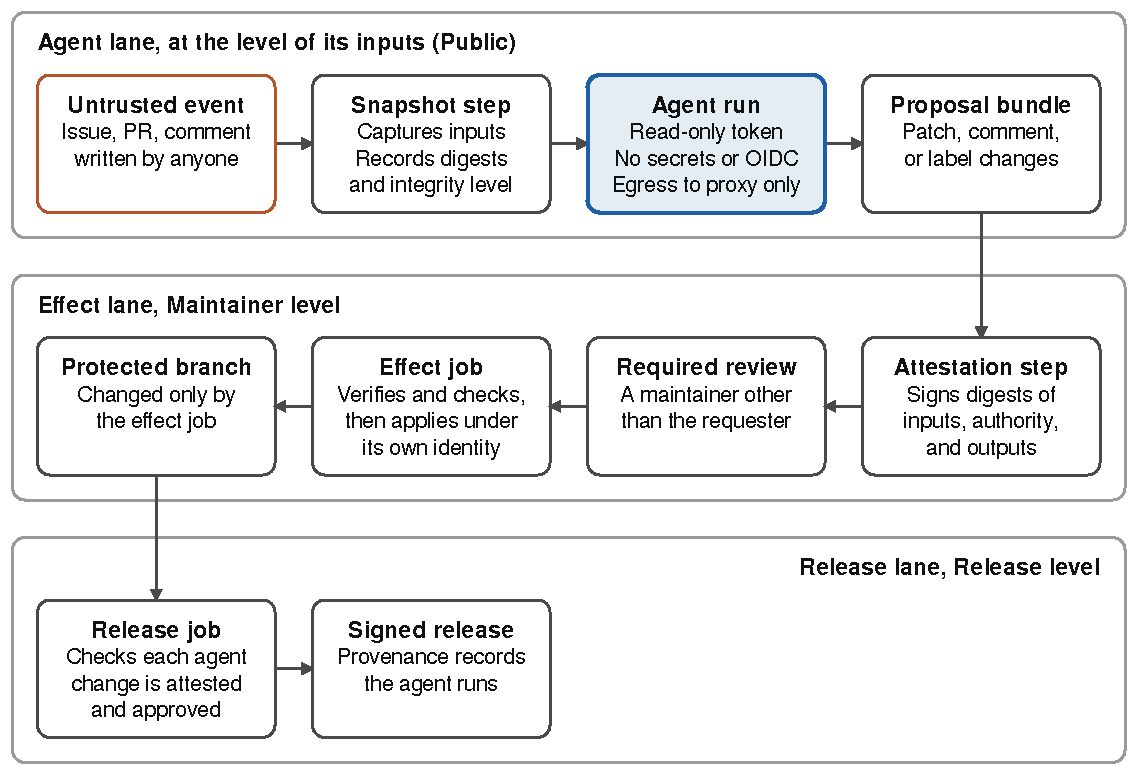
\includegraphics[width=\linewidth]{figures/fig2-three-lanes.pdf}
\caption{The agent lane runs at the integrity level of its inputs and produces only proposals. Approved, deterministic jobs apply them, and the release lane verifies attestations and approvals before publishing. Agent instruction files are read from the protected base branch, and the model credential stays in the inference proxy.}
\Description{A diagram of three horizontal lanes. In the agent lane, an untrusted event feeds a snapshot step, an agent run with a read-only token and no secrets, and a proposal bundle. In the effect lane, an attestation step, a required review by another maintainer, and an effect job lead to a protected branch. In the release lane, a release job checks that each agent change is attested and approved before producing a signed release whose provenance records the agent runs.}
\label{fig:2}
\end{figure}


\subsection{Realization on GitHub Actions}\label{sec:7.2}

Most of the required primitives exist today. Job-level permissions and per-job tokens bound authority (R2, R3). OIDC claims bind cloud credentials to a repository, ref, environment, and workflow~\cite{githubndopenid}. Environments with required reviewers and self-review prevention implement the approval in R4~\cite{githubnddeployments}. Branch rulesets with code-owner review, and on paid plans push rulesets that block changes to listed file paths, protect the instruction plane (R5)~\cite{githubndabout}. The attest action signs custom in-toto predicates (R8)~\cite{githubndactions}.

Two gaps remain. GitHub-hosted runners provide a new virtual machine for each job~\cite{githubndgithub} but no native egress allow-list. R7 therefore needs either self-hosted ephemeral runners with network policy, or a runtime monitor of the kind that first detected the tj-actions compromise through an unexpected outbound connection~\cite{stepsecurity2025harden}. And no platform today derives permissions from input provenance, so R1 and R2 are implemented by structure, with a separate workflow per lane, rather than by policy.

Vendors are converging on parts of this design. GitHub's Copilot cloud agent pushes only to its own branch, cannot approve or merge its own pull requests, does not trigger workflows on them until a user with write access approves, restricts internet access with a firewall, and never presents comments from users without write access to the agent~\cite{githubndrisks}. The Claude Code action accepts triggers only from users with write access and restores agent configuration files from the base branch in workflows triggered by pull\_request\_target or workflow\_run~\cite{anthropicndsecurity}. An industry research note from May 2026 recommends separating agent decision-making from the execution layers that hold credentials~\cite{cloud2026prompt}. Our contribution is to state the principle these practices share, to show which incidents each control addresses, and to add the pieces they lack: provenance-based labels, snapshot binding, and attestation of agent runs.


\subsection{The agent-run attestation}\label{sec:7.3}

Table~\ref{tab:3} lists the fields of the proposed attestation. It is an in-toto statement whose subject is the proposal bundle and whose predicate type is a project-defined URI. The design follows SLSA's rule that provenance must not be forgeable by user-defined steps~\cite{openndslsa}: fields the agent could influence are kept apart and marked untrusted.

\begin{table}[htbp]
\caption{Fields of the agent-run attestation.}
\label{tab:3}
\footnotesize
\begin{tabularx}{\linewidth}{@{}>{\hsize=0.527\hsize\raggedright\arraybackslash}X>{\hsize=2.251\hsize\raggedright\arraybackslash}X>{\hsize=0.694\hsize\raggedright\arraybackslash}X>{\hsize=0.527\hsize\raggedright\arraybackslash}X@{}}
\toprule
\textbf{Field} & \textbf{Content} & \textbf{Produced by} & \textbf{Trusted} \\
\midrule
Subject & Digests of the proposal bundle files & Attestation step & Yes \\
Trigger & Event type and identifier, repository, triggering principal and level & Snapshot step & Yes \\
Inputs & Each snapshot item with digest, channel, and label; the computed integrity level & Snapshot step & Yes \\
Authority & Token permissions, names of secrets granted, network policy, OIDC permission & Protected workflow definition and snapshot step & Yes \\
Agent & Digests of the action and harness; model identifier and version as reported by the inference proxy & Snapshot step and proxy & Yes \\
Trace & Tool calls with digests of their arguments & Agent harness & No (self-reported) \\
Approvals & Reviewer identity, time, and environment & Effect lane & Yes \\
\bottomrule
\end{tabularx}
\end{table}


\section{Analytical evaluation}\label{sec:8}

We evaluate the design in four ways: by whether it would have prevented or contained the outcomes in \S\ref{sec:4}, by traceability to existing standards, by deployability on GitHub Actions, and by the risk it leaves behind. The evaluation is analytical. Section~\ref{sec:9} describes the empirical study needed to confirm it.


\subsection{Incident coverage}\label{sec:8.1}

Under the assumptions of \S\ref{sec:5.3}, the requirements would have prevented the harmful outcome in eight of the ten cases, would have prevented or contained it in one depending on how the poisoned file entered the project, and would have contained it in one (Table~\ref{tab:4}). \emph{Prevented} means the outcome could not occur. \emph{Contained} means the injected behavior could still occur but could not reach the asset the attacker wanted.

\begin{table}[htbp]
\caption{Requirements that would have prevented (P) or contained (C) each outcome.}
\label{tab:4}
\footnotesize
\begin{tabularx}{\linewidth}{@{}>{\hsize=0.751\hsize\raggedright\arraybackslash}X>{\hsize=0.588\hsize\raggedright\arraybackslash}X>{\hsize=0.588\hsize\raggedright\arraybackslash}X>{\hsize=2.073\hsize\raggedright\arraybackslash}X@{}}
\toprule
\textbf{Case} & \textbf{Prevented by} & \textbf{Contained by} & \textbf{Reasoning} \\
\midrule
Rules File Backdoor & R5 (if the file entered through review) & R4, R8 & A hidden-character scan and code-owner review block the poisoned file; agent output stays a reviewable, labeled proposal. \\
GitHub MCP & R2 & R1, R3 & An invocation that reads a public issue holds no read access to private repositories. \\
GitLab Duo & R2 & R7 & Context written by other users bounds the assistant's read access; rendering-based channels are closed. \\
Gemini CLI & - & R2, R7 & The injected command still runs, but finds no secrets and no route out. \\
Amazon Q extension & R3, R4, R5 & R8 & A job-scoped token cannot write the source repository; agent instructions require code-owner review; release verification flags unattested changes. \\
Nx ``s1ngularity'' & R1, R2, R3, R4 & R8 & The pull-request title is Public input to a Maintainer-level job; tokens default to read-only; publication requires OIDC and approval. \\
CamoLeak & R2 & R7 & As for GitLab Duo: the proxy channel is irrelevant when private data is out of reach. \\
PromptPwnd & R2, R3 & R4, R7 & Agents that read issue text hold no secrets or write tokens, and model keys sit behind a proxy. \\
Claude Code action & R1 & R2 & The snapshot fixes the title when authority is decided, and a run influenced by the public holds no secrets. \\
Clinejection & R7 & R2, R3, R8 & A run triggered by an issue shares no writable cache with release jobs, so code it runs cannot reach release credentials; per-release credentials issued through OIDC limit what a theft yields. \\
\bottomrule
\end{tabularx}
\end{table}

The Nx case shows that the principle is not specific to LLMs. Interpolating a pull-request title into a privileged shell step is the same input–authority mismatch, with a shell in place of a model.

\emph{Threats to validity.} This is a retrospective, counterfactual analysis of public reports. It is open to hindsight bias, the reports may omit relevant details, and incidents that were never disclosed are absent. The prevention claims also assume each requirement is implemented correctly.


\subsection{Traceability to standards}\label{sec:8.2}

Table~\ref{tab:5} maps each requirement to the topics of the NCCoE concept paper~\cite{booth2026accelerating}, to SSDF practices~\cite{souppaya2022secure,booth2025secure}, and to SLSA v1.2~\cite{openndslsa}. SP 800-204D's guidance on attestations and provenance in CI/CD pipelines~\cite{chandramouli2024strategies} covers the mechanism of R8 but not its agent-specific fields.

\begin{table}[htbp]
\caption{Traceability of the requirements.}
\label{tab:5}
\footnotesize
\begin{tabularx}{\linewidth}{@{}>{\hsize=0.924\hsize\raggedright\arraybackslash}X>{\hsize=1.119\hsize\raggedright\arraybackslash}X>{\hsize=0.681\hsize\raggedright\arraybackslash}X>{\hsize=1.036\hsize\raggedright\arraybackslash}X>{\hsize=1.240\hsize\raggedright\arraybackslash}X@{}}
\toprule
\textbf{Requirement} & \textbf{NCCoE topic} & \textbf{SSDF practice} & \textbf{SLSA v1.2} & \textbf{What is new} \\
\midrule
R1 & Prompt-injection controls & None & None & Trust labels for content an automated actor reads \\
R2 & Authorization; prompt-injection controls & PO.5 & Build L3: secrets inaccessible to user-defined steps & Labels determine permissions \\
R3 & Identification; authorization & PO.5 & Build provenance identifies the builder & A distinct identity per agent invocation \\
R4 & Authorization & PS.1, PW.7 & Source L4: two-party review & Approval of agent proposals by someone other than the requester \\
R5 & Prompt-injection controls & PS.1 & Source L3: continuous technical controls & Agent instruction files treated as code \\
R6 & None & PO.3, PW.4 & Verification of artifact provenance & Tool descriptions treated as untrusted input \\
R7 & Prompt-injection containment & PO.5 & Build L3: isolated, ephemeral environments & Default-deny egress for agents \\
R8 & Auditing; non-repudiation & PS.2, PS.3 & Build provenance (L2–L3) & An agent-run predicate \\
\bottomrule
\end{tabularx}
\end{table}

Two findings stand out. First, R1 has no counterpart in the SSDF or SLSA: neither framework has a notion of the trust level of text that an automated actor reads. Second, the NCCoE's questions on identification, authorization, auditing, and non-repudiation~\cite{booth2026accelerating} map onto R3, R2 and R4, and R8, which suggests the agent-run attestation as a concrete artifact that a demonstration project could build.


\subsection{Deployability on GitHub Actions}\label{sec:8.3}

Table~\ref{tab:6} lists, for each requirement, the GitHub Actions primitive that realizes it today and the gap that remains, with a compensating control for each gap.

\begin{table}[htbp]
\caption{Native support for each requirement, and the remaining gap.}
\label{tab:6}
\small
\begin{tabularx}{\linewidth}{@{}>{\hsize=0.580\hsize\raggedright\arraybackslash}X>{\hsize=1.210\hsize\raggedright\arraybackslash}X>{\hsize=1.210\hsize\raggedright\arraybackslash}X@{}}
\toprule
\textbf{Requirement} & \textbf{Native primitive} & \textbf{Gap and compensating control} \\
\midrule
R1 & Event payloads identify authors; workflows can be split by trust & No provenance labels or snapshot binding; implement as a deterministic step before the agent \\
R2 & Job-level permissions; environment secrets released only after approval \cite{githubnddeployments} & No policy engine maps labels to permissions; enforce through lane structure and organization policy \\
R3 & Job tokens that expire with the job \cite{anthropicndsecurity}; per-job OIDC tokens with claims \cite{githubndopenid} & Cloud trust policies must constrain the claims \cite{cloud2026prompt}; model keys need a proxy \\
R4 & Environments with required reviewers and self-review prevention \cite{githubnddeployments}; branch rulesets & Deterministic checks on proposals are project-defined \\
R5 & Code owners and branch rulesets; push rulesets that restrict file paths, on paid plans for private repositories \cite{githubndabout} & Hidden-character scanning is project-defined, though GitHub now warns about hidden Unicode \cite{pillar2025new} \\
R6 & Referencing actions by full commit digest & No native verification of an action's provenance when it is consumed \\
R7 & A new virtual machine for each job on GitHub-hosted runners \cite{githubndgithub} & No native egress allow-list; use self-hosted ephemeral runners with network policy, or a runtime monitor \cite{stepsecurity2025harden} \\
R8 & The attest action with custom predicates \cite{githubndactions} & Agent-specific fields are project-defined \\
\bottomrule
\end{tabularx}
\end{table}


\subsection{Residual risk}\label{sec:8.4}

\begin{itemize}
\item \emph{Harm at the adversary's own level.} An agent can still post misleading comments, generate noise, or consume budget. Deterministic output filters, rate limits, and spending caps bound these effects.
\item \emph{Endorsement failure.} Approvers may miss malicious changes in an agent's proposal. Manual security review is unreliable: in one study, none of 30 developers found all seven known vulnerabilities in a small application~\cite{edmundson2013empirical}. R8 makes agent-authored changes identifiable, so that they can receive added scrutiny.
\item \emph{Labeling errors.} Under-labeling voids the proposition, and over-labeling costs utility. Labels must reflect repository settings, such as who may comment or open pull requests.
\item \emph{Ambient authority.} Persisted checkout credentials~\cite{githubndactionsa}, shared caches, and metadata endpoints must be removed explicitly; their presence violates assumption (i).
\item \emph{Private repositories.} Where only collaborators can write issues, the lowest influencing level rises to Contributor, and more automation is safe.
\item \emph{Utility.} Some current agent features, such as pushing directly to protected branches, become two-step processes.
\end{itemize}


\section{Protocol for empirical evaluation}\label{sec:9}

The analysis above rests on stated assumptions and on public reports. We will test it with a controlled study and pilot deployments, organized around three research questions.

\textbf{RQ1 (security).} Does the three-lane architecture prevent privileged effects under adaptive prompt injection? We will build a suite of CI tasks (issue triage, code review, build repair, and dependency updates) and inject attacks through each channel of \S\ref{sec:3.1}, using the sources and sinks catalogued by Wang et al.~\cite{wang2026demystifying} and AgentDojo's method of pairing each utility task with security test cases~\cite{debenedetti2024agentdojo}. Attacks will be adapted to each configuration, following Nasr et al.~\cite{nasr2025attacker}. Each task runs under three configurations:

\begin{itemize}
\item \emph{B0:} the vendor's default configuration for the agent action.
\item \emph{B1:} a hardened single-workflow configuration, with least-privilege tokens and write-access trigger checks.
\item \emph{T:} the three-lane architecture of \S\ref{sec:7}.
\end{itemize}

Seeded canary credentials and protected refs make outcomes observable. The primary measure is the rate of privileged effects: canary disclosure, writes to protected refs, changes to instruction files, and publication. The secondary measure is the rate of effects at the adversary's own level, such as misleading comments. We hypothesize that T yields no privileged effects, by construction, and that B0 and B1 yield some.

\textbf{RQ2 (utility and cost).} What does the architecture cost the people who use it? We will compare B1 and T on task success rate, time from trigger to merged change, approvals per change, reviewer time per approval, and CI minutes consumed.

\textbf{RQ3 (deployability).} How much effort does adoption take? We will measure the configuration changes and setup time needed in pilot deployments, including independent game studios recruited through the OBAAF pilot program described in the companion paper~\cite{keluoudeke2026securing}.

\emph{Ethics.} Experiments will use only repositories we control or whose owners consent in writing, synthetic canary secrets rather than real credentials, and coordinated disclosure for any vendor flaw found during the study.


\section{Related work}\label{sec:10}

\emph{Prompt injection and model-level defenses.} Indirect prompt injection was characterized against real applications by Greshake et al.~\cite{greshake2023not}, and OWASP lists it as the leading risk for LLM applications~\cite{owaspndowasp}. AgentDojo provides a dynamic benchmark of attacks and defenses for agents~\cite{debenedetti2024agentdojo}. Defenses that mark untrusted input~\cite{hines2024defending} or train an instruction hierarchy into the model~\cite{wallace2024instruction} reduce attack success, but adaptive attacks bypass most published defenses~\cite{nasr2025attacker}. Our design assumes these defenses may fail.

\emph{System-level agent defenses.} A growing body of work enforces security outside the model. CaMeL extracts control and data flow from the trusted query and attaches capabilities to data, solving 77\% of AgentDojo tasks with provable security against 84\% for an undefended agent~\cite{debenedetti2025defeating}. Beurer-Kellner et al. catalog design patterns, such as plan-then-execute and the dual LLM, that keep untrusted input from triggering consequential actions~\cite{beurerkellner2025design}. Fides tracks confidentiality and integrity labels through an agent's planner~\cite{costa2025securing}. Progent enforces programmable privilege policies on tool calls~\cite{shi2025progent}, IsolateGPT isolates the execution of third-party applications in agentic systems~\cite{wu2025isolategpt}, and CapScope replaces ambient authority in coding agents with capability scopes minted from trusted input~\cite{bouras2026authority}. These systems enforce policy inside the agent runtime and are evaluated on general agent tasks. Our work enforces policy at the orchestration layer of build pipelines, using identities and permissions the CI platform already enforces. It derives authority from the provenance of all inputs rather than from the user's request alone, and it adds agent runs to the provenance of the software supply chain. The approaches compose: a pipeline built on taint-bounded authority can host any of these agents in its agent lane (\S\ref{sec:5.4}).

\emph{CI/CD security.} Koishybayev et al. measured pervasive over-privilege in GitHub workflows~\cite{koishybayev2022characterizing}. ARGUS found code injection flaws through staged taint analysis~\cite{muralee2023argus}, and Gu et al. characterized threats across CI services~\cite{gu2023continuous}. GitHub's own guidance on untrusted pull requests introduced the split between unprivileged and privileged workflows that our lanes generalize~\cite{lobavcevski2021keeping}. Closest to our setting, Wang et al. defined agentic workflow injection and built a static taint analyzer for it~\cite{wang2026demystifying}. Their tool finds the violations; our requirements give the architectural remedy that removes the class. A May 2026 industry note reaches several of the same recommendations from practice~\cite{cloud2026prompt}.

\emph{Supply chain integrity.} in-toto~\cite{torresarias2019toto}, Sigstore~\cite{newman2022sigstore}, SLSA~\cite{openndslsa}, the SSDF~\cite{souppaya2022secure,booth2025secure}, and SP 800-204D~\cite{chandramouli2024strategies} provide the provenance, signing, and integrity levels on which R8 builds. Systematizations by Ladisa et al.~\cite{ladisa2023sok} and Okafor et al.~\cite{okafor2022sok} frame the attack space and the design properties of transparency, validity, and separation. Agents add an actor these frameworks do not yet model: one whose behavior is a function of untrusted text.

\emph{Integrity and authority models.} Our principle adapts Biba's low-water-mark policy~\cite{biba1977integrity} and uses Clark and Wilson's certified transformations for endorsement~\cite{clark1987comparison}. It applies Saltzer and Schroeder's least privilege and complete mediation~\cite{saltzer1975protection} and removes Hardy's confused deputy~\cite{hardy1988confused}, within Denning's lattice view of information flow~\cite{denning1976lattice}. Willison's ``lethal trifecta'' of private data, untrusted content, and external communication~\cite{willison2025lethal} is the confidentiality case of taint-bounded authority.


\section{Limitations}\label{sec:11}

\begin{itemize}
\item \emph{The evaluation is analytical.} We have argued what the requirements would have done and shown that they can be built; we have not yet measured them. Section~\ref{sec:9} describes the study that will.
\item \emph{The incident corpus is small and public.} Ten cases cannot represent everything that has happened. Public reports favor issues that researchers found and vendors acknowledged, and our coverage analysis is counterfactual.
\item \emph{The realization is GitHub-specific.} GitLab CI, Jenkins, and other platforms offer analogous primitives (job tokens, protected environments, OIDC, ephemeral runners), but we have not evaluated them.
\item \emph{The trust model is simplified.} Four levels in a chain do not capture bots, organization-wide roles, per-path ownership, or trust that spans repositories. Extending to a richer lattice is straightforward in principle, but it is not evaluated here.
\item \emph{Confidentiality is handled conservatively.} Treating every read of private data as a capability withholds data that a particular invocation could safely use. Finer-grained policies are possible, at the cost of more complex labeling.
\item \emph{Human approval is assumed, not modeled.} The endorsement step depends on approvers whose error rates we discuss (\S\ref{sec:8.4}) but do not model.
\item \emph{Some threats are out of scope.} These include compromise of model providers, poisoning of training data, and compromise of developer endpoints.
\end{itemize}


\section{Conclusion}\label{sec:12}

Agents bring a new kind of actor into build pipelines: one that cannot reliably distinguish the text it reads from the instructions it follows. We argued that the safe response is to stop requiring it to. Taint-bounded authority bounds what an agent invocation can do by who could have written what it reads. A three-lane architecture enforces that bound with controls CI platforms already provide, and an agent-run attestation records each run in the provenance of the software it helped produce. Our analysis of ten documented incidents suggests these controls would have prevented most of the outcomes and contained the rest. The next step is to measure their cost and residual risk in real pipelines, beginning with the study and pilots described in \S\ref{sec:9}. These controls form OBAAF's agent-assurance component, and the companion paper incorporates them into the framework's build-assurance profile for video game studios.

\begin{acks}
To be added by the author.

\end{acks}

\bibliographystyle{ACM-Reference-Format}
\bibliography{refs}

\end{document}
